\chapter{Introducción}
\label{cap:Introduccion}

Este capítulo aborda la motivación del trabajo. Se trata de señalar la necesidad de la que surge, su actualidad y pertinencia. Puede incluir también un estado de la cuestión en la que se revisen estudios o desarrollos previos y en qué medida sirven de base al trabajo que se presenta.

A continuación se muestran algunos ejemplos para la inclusión de elementos en el documento.

% ------------------------------------------------------------------------------
% Ejemplos para la plantilla
% ------------------------------------------------------------------------------
\section{Ejemplos de listas}
\label{sec:ejListas}
\index{ejemplos} % Véase cómo se incluyen entradas en el índice alfabético
A continuación se van a añadir algunos ejemplos que pueden emplearse al redactar la memoria.

\index{ejemplos!listas} % Para el índice
\noindent Ejemplo de lista con \emph{bullet} especial. 
% Ejemplo: Lista con bullets especiales
% ============
\begin{itemize}
	\item[*] peras
	\item manzanas
	\item[\ding{170}] naranjas
\end{itemize}

\noindent Ejemplo de lista compacta (también se puede emplear el entorno para enumeraciones \emph{compactenum})
% Ejemplo: Lista con balas
% ============
\begin{compactitem}
	\item peras
	\item manzanas
	\item naranjas
\end{compactitem}


\noindent Ejemplo de lista en varias columnas.
% Ejemplo: Listas en varias columnas
% ============
\begin{multicols}{2} % El parámetro es el número de columnas de la lista
	\begin{compactenum}
		\item peras
		\item manzanas
		\item naranjas
		\item patatas
		\item calabazas
		\item fresas
	\end{compactenum}
\end{multicols}


\newpage


\section{Ejemplos de tablas}
\label{sec:ejTablas}
\index{ejemplos!tablas}
A continuación se incluyen algunos ejemplos de tablas hechas con \LaTeX{} y paquetes dedicados.

% Ejemplo: Tabla con macro \cline
% ==========
\begin{table}[htb]%
	\centering
	\caption{Ejemplo de uso de la macro \texttt{cline}}
	\label{tab:cline}
	\begin{tabular}[t]{|r|l|}
		\hline
		7C0 & hexadecimal \\[1cm] % Ejemplo de separación fijada entre líneas
		3700 & octal \\ \cline{2-2}
		11111000000 & binario \\
		\hline \hline
		1984 & decimal \\
		\hline
	\end{tabular}
\end{table}


\noindent Ejemplo de tabla en la que se controla el ancho de la celda.

% Ejemplo: Ejemplo de tabla con control de la anchura de celda.
% ==========
\begin{table}[htb]%
	\centering
	\caption{Ejemplo de tabla con especificación de anchura de columna}
	\label{tab:anchura}
	\begin{tabular}{ | l | l | l | p{5cm} |}
		\hline
		Día & Temp Mín (\textdegree C) & Temp Máx (\textdegree C) & Previsión \\ \hline
		Lunes & 11 & 22 & Día claro y muy soleado. Sin embargo, la brisa de la tarde puede hacer que las temperaturas desciendan \\ \hline
		Martes & 9 & 19 & Nuboso con chubascos en muchas regiones. En Cataluña claro con posibilidad de bancos nubosos al norte de la región \\ \hline
		Miércoles & 10 & 21 & La lluvía continuará por la mañana pero las condiciones climáticas mejorarán considerablemente por la tarde\\
		\hline
	\end{tabular}
\end{table}

\clearpage


\section{Ejemplos de figuras}
\label{sec:ejFiguras}
\index{ejemplos!figuras}

En esta sección se añaden ejemplos de muestra para la inclusión de figuras simples y subfiguras.

% Ejemplo: Ejemplo de inclusión de figura
% ============
\begin{figure}[htb]
	\centering
	
\includegraphics[width=0.4\linewidth]{escudoInf}
	\caption[Ejemplo de figura]{Figura vectorial del escudo de la ESI}
	\label{fig:ejFigure}
\end{figure}


\noindent Ejemplo de figuras compuestas por subfiguras.

% Ejemplo: Ejemplo de inclusión de subfiguras
% ============
\begin{figure}[htb]
	\centering
	\subfigure[Gráfico vectorial PDF]{
		
\includegraphics[width=0.4\linewidth]{escudoInf}
		\label{fig:escudoColor}
	} 
	\subfigure[Gráfico png]{
		
\includegraphics[width=0.4\linewidth]{escudoInfBW}
		\label{fig:escudoBW}
	}
	\caption[Ejemplo de subfiguras]{Ejemplo de inclusión de subfiguras en un mismo entorno}
	\label{fig:ejSubfigures}
\end{figure}


\clearpage


\section{Ejemplos de listados}
\label{sec:ejListados}
\index{ejemplos!listados}

Ejemplos más representativos de inclusión de porciones de código fuente.

% Ejemplo: Listado Java
% ============
\begin{lstlisting}[language=Java,float=ht,caption={[Código fuente en Java]Ejemplo de código fuente en lenguaje Java},label=lst:java]
// @author www.javadb.com
public class Main {    
// Este método convierte un String a
// un vector de bytes

public void convertStringToByteArray() {

String stringToConvert = "This String is 15";      
byte[] theByteArray = stringToConvert.getBytes();        
System.out.println(theByteArray.length);        
}

// argumentos de línea de comandos 
public static void main(String[] args) {
new Main().convertStringToByteArray();
}
}
\end{lstlisting}



\noindent Otro ejemplo.

\begin{lstlisting}[style=C-ruled,float=ht,caption={Ejemplo de código C},label=lst:codC]
// Este código se ha incluido tal cual está 
// en el fichero \LaTeX{}
#include <stdio.h>
int main(int argc, char* argv[]) {
puts("¡Hola mundo!");
}
\end{lstlisting}


\noindent Ejemplo de entrada por consola.

\begin{lstlisting}[style=consola, numbers=none]
$ gcc -o Hola HolaMundo.c
\end{lstlisting}


\subsection{Algoritmos con el paquete \texttt{algorithm2e}}
Como ya se ha comentado en los textos científicos relacionados con las TIC\footnote{Por supuesto en un TFG o tesis de una Escuela de Informática.} (Tecnologías de la Información y Comunicaciones) suelen aparecer porciones de código en los que se explica alguna función o característica relevante del trabajo que se expone. Muchas veces lo que se quiere ilustrar es un algoritmo o método en que se ha resuelto un problema abstrayéndose del lenguaje de programación concreto en que se realiza la implementación. El paquete \texttt{algorithm2e}\footnote{\url{https://osl.ugr.es/CTAN/macros/latex/contrib/algorithm2e/doc/algorithm2e.pdf}} proporciona un entorno \texttt{algorithm} para la impresión apropiada de algoritmos tratándolos como objetos flotantes y con muchas flexibilidad de personalización. En el algoritmo \ref{alg:como} se muestra cómo puede emplearse dicho paquete. En este curso no se explican las posibilidades del paquete más en profundidad ya que excede el propósito del curso. A todos los interesados se les remite a la documentación del mismo.


% Ejemplo:
% ============
\IncMargin{1em}
\begin{algorithm}
\SetKwInOut{Input}{Datos}\SetKwInOut{Output}{Resultado}
\LinesNumbered
\SetAlgoLined

\Input{este texto} 
%\KwIn{este texto}
\Output{como escribir algoritmos con \LaTeX2e}
%\KwOut{como escribir algoritmos con \LaTeX2e}

inicialización\;
\While{no es el fin del documento}{
	leer actual\;
	\eIf{comprendido}{
		ir a la siguiente sección\;
		la sección actual es esta\;
	}{
		ir al principio de la sección actual\;
	}
}

% Aunque el captión aparece abajo siempre se pone arriba como en tablas y listados
\caption{Cómo escribir algoritmos}\label{alg:como}
\end{algorithm}\DecMargin{1em}

\newpage

\section{Menús, paths y teclas con el paquete \texttt{menukeys}}
Cada vez es más usual que los trabajos en ingeniería exijan el uso de software. Para poder especificar de modo elegante el uso menús, pulsación de teclas y directorios se recomienda el uso del paquete \texttt{menukeys}.\footnote{\url{https://osl.ugr.es/CTAN/macros/latex/contrib/menukeys/menukeys.pdf}} Este paquete nos permite especificar el acceso a un menú, por ejemplo:

\menu{Herramientas > Órdenes > PDFLaTeX}\\

\noindent También un conjunto de teclas. Por ejemplo:
\keys{\ctrl + \shift + T}\\

\noindent O un directorio:
\directory{C:/user/LaTeX/Ejemplos}\\

\noindent Aunque este paquete permite muchas opciones de configuración de los estilos aplicados, no es necesario hacerlo para obtener unos resultados muy elegantes.
















Descripción esgrima

La esgrima es un deporte de estrategia en el cuál tendrás que analizar a tu
 oponente a la vez que te defiendes de sus acometidas. A la vez, tendrás que
 disfrazar tus ataques con otros para que el oponente no sea capaz de analizar
 tus movimientos. Es por esto por lo que la mayoría de practicantes lo denominan
 el ajedrez en movimiento puesto que todo son ataques, por un franco u otro,
 pequeñas batallas que te llevarán a ganar la guerra al final. Jugar con la mente
 del rival y calmar la tuya para tener superioridad táctica.

Por supuesto que el físico influye en este deporte, no deja de ser un deporte de contacto
 en el cual las cualidades físicas (fuerza, agilidad, rapidez, coordinación, reflejos, etc)
 son un factor mas a tener en cuenta, pero esto no serán mas que componentes de una ecuación
 la cual nos dará la victoria.

Al ser un deporte minoritario, que alguna vez hemos visto en la televisión cuando hay
 olimpiadas y nos detenemos un momento a verlo porque hay espadas y vemos a dos personas
 luchando con ellas como si de piratas o de mosqueteros se tratasen, pasemos a explicar por encima
 en que consiste un asalto de esgrima. Un asalto de esgrima es un enfrentamiento entre dos
 oponentes los cuales tienen que llegar al límite de tocados antes que el rival o estar por encima
 de este una vez haya terminado el tiempo de asalto. Dependiendo de la modalidad y categoría
 variaran estos tiempos y límite de tocados. ¿Pero que es un tocado? Un tocado no es mas que
 un punto a tu favor, el cual se puede conseguir tocando al rival o mediante sanciones del rival.
 Un ejemplo de sanciones podría ser un comportamiento antideportivo, salirse de la pista por el fondo,
 dar varias veces la espalda, perder el tiempo repetidas veces mientras vas perdiendo, etc.

Como la mayoría de artes marciales no es mas que un esquema táctico en el cuál tendremos unas variables
 de entrada mediante las cuales determinaremos una salida. ¿Pero como es posible que un deporte de contacto
 se base en una serie de entradas y salidas? Bien, un ejemplo muy básico es el siguiente: ante una acción ofensiva
 directa hacia la parte superior del cuerpo lo lógico es cubrirse esta parte. Aquí es donde entra en juego
 la estrategia de cada componente del combate. Si el atacante sabe que tu reacción ante una amenaza arriba
 será cubrirte esa zona, el amagará con un ataque falso (finta) a una parte del cuerpo y sobre tu acción
 defensiva para evitar esta acometida aprovechará para atacar otra zona que dejaste descubierta por
 defender la primera acción. Por otro lado, el defensor puede analizar al rival y saber que el primer ataque
 no será el verdadero, si no que será una preparación para atacar sobre otra zona, de este modo anticiparse
 y atacar sobre esta preparación o amagar con defenderse sobre la primera zona para después cubrirse la segunda
 y contra-atacar.

Una vez tenemos unas nociones básicas sobre como funciona un esquema táctico en general sobre cualquier
 disciplina de arte marcial o deporte de contacto, pasemos a hablar de la esgrima en concreto.
 Hay tres disciplinas dentro de este deporte: sable, florete y espada. Siendo la primera una modalidad
 en la que se puede tocar con cualquier parte de la hoja, mientras que en las dos últimas son armas de
 estoque, es decir, solo vale tocar con la punta. Puesto que cada modalidad tiene unas normas y la espada
 es la mas practicada y mas sencilla de todas, nos centraremos en ella. En la modalidad de espada se puede
 tocar en cualquier parte del cuerpo, esto incluye desde el pecho, hasta la suela de la zapatilla, pasando
 por la espalda o cualquier lugar que se nos ocurra. Con la única excepción de la nuca, puesto que es la única
 zona en la que no hay protección, para ello hay normas evitando que des la espalda y expongas esta zona
 tan delicada.

% https://es.m.wikipedia.org/wiki/Archivo:Fencing_epee_valid_surfaces.svg
\begin{figure}[htb]
	\centering
	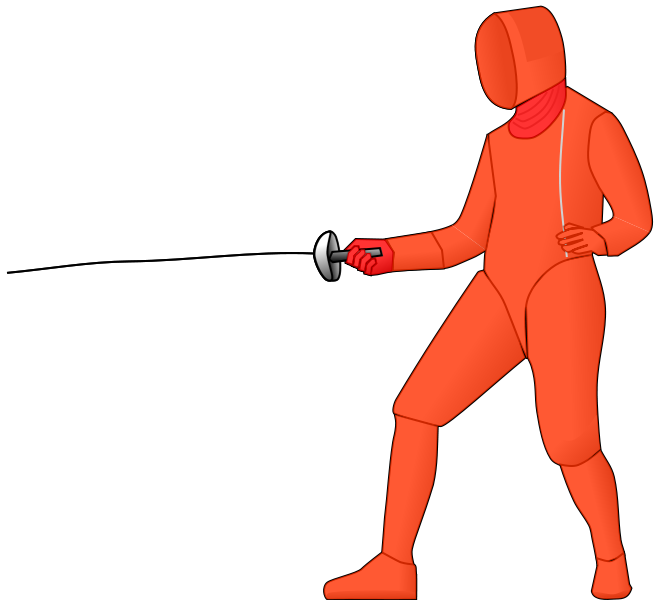
\includegraphics[width=0.4\linewidth]{blancoValido}
	\caption[Blanco válido espada]{Blanco válido espada}
	\label{fig:blancoValido}
\end{figure}

Como hemos mencionado antes es un arma de estoque, por lo que el mecanismo de activación estará en la punta
 y será mediante un botón, el cuál al presionarse sobre un blanco válido cerrará un circuito electrico cuyo
 objetivo es señalizar el tocado. A partir de este momento el rival tiene un breve periodo de tiempo, 0.4 segundos,
 para realizar un tocado sobre el rival y que haya un tocado doble. Pasado este tiempo el circuito se bloqueará
 y solo habrá un tocado válido. A pesar de que haya un tocado doble no quiere decir que siempre sean válidos
 ambos tocados. Mediante las normas se dictaminará si los dos lo son, solo uno o ninguno de ellos lo es.
 Un ejemplo podría ser que uno de los dos tiradores se encuentre fuera de la pista, lo cual anularía su tocado.
 Como se han podido dar cuenta, hemos hablado de tiempo, por lo que otro componente a tener en cuenta es ser mas
 rápido que el rival, esto habrá que tenerlo en cuenta en nuestro esquema táctico para poder decidir una acción en
 la cual, aunque nos toquen, nosotros lo hagamos con suficiente antelación al rival de modo que su tocado no
 sea válido. Tal y como se habló antes los asaltos tienen un límite de tiempo y un límite de tocados,
 este será otro factor a tener en cuenta en nuestro esquema táctico sobre como plantear el asalto.
 Puede que a veces nos interese llevar un asalto hasta el final del tiempo desgastando físicamente al
 rival para aprovechar esta superioridad al final. Otras veces quizás nos interese lo contrario,
 acabar con el asalto cuanto antes para evitar dejar al contrario pensar. Puede que otras veces nos
 interese alargar el asalto al mayor número de tocados posibles puesto que tengamos mayor
 repertorio que nuestro oponente, mientras que en el caso contrario, si tenemos pocas acciones nos interesará
 hacer el menor número de tocados. También habrá que tener en cuenta el marcador y cuanta distancia hay
 hasta el final del combate, si al rival le falta un tocado para ganar, mientras que a nosotros nos faltan
 tres, no nos interesa que haya un tocado doble puesto que el ganaría. Estas son algunas de las variables
 entran dentro de la formula para plantear nuestra táctica en un asalto de esgrima.

Una vez que ya sabemos como funciona un asalto de esgrima podemos hablar sobre como funciona una competición
 de esgrima. Primero hablaremos de las individuales y mas tarde de los equipos. Se explicará el funcionamiento
 de una competición estandar, lo cual puede variar en función de la categoría y tipo de competición.
 En cuanto a las competiciones individuales primero se disputa una fase de grupos, la cual se denomina
 \textit{poule} en la cual se dividen a todos los tiradores en poules (grupos) de seis o siete tiradores en función
 del número de participantes que haya. Siendo siete el número ideal y dejando las de seis en caso de que
 no haya número suficiente de tiradores. Estas poules se hacen en función del ranking de los tiradores inscritos
 a la competición, de manera que estén lo mas equilibradas posibles. Una vez organizadas los poules se da
 comienzo a ellas. En ellas se enfrentan todos los tiradores entre ellos, empezando los que sean del mismo
 país y club, para evitar favoritismos mas adelante. Estos enfrentamientos serán en un único asalto con un
 límite de cinco tocados y una duración máxima de tres minutos. El primero que llegue al límite con diferencia
 de un tocado o quien tenga mayor puntuación al acabar el tiempo será el ganador de este encuentro.

\begin{table}[htb]%
  \centering
  \caption{Ejemplo tabla resultados poule}
  \label{tab:anchura}
  \begin{tabular}{ | l | l | l | l | l | l | l | l | }
    \hline
    & Tirador 1 & Tirador 2 & Tirador 3 & Tirador 4 & Tirador 5 & Tirador 6 & Tirador 7 \\ \hline
    Tirador 1 & x & V & & & & & \\ \hline
    Tirador 2 & 1 & x & & & & & \\ \hline
    Tirador 3 & & & x & & & & \\ \hline
    Tirador 4 & & & & x & & & 2 \\ \hline
    Tirador 5 & & & & & x & & \\ \hline
    Tirador 6 & & & & & & x & \\ \hline
    Tirador 7 & & & & $V_3$ & & & x \\
    \hline
  \end{tabular}
\end{table}

La anterior tabla sería un ejemplo de una tabla de poule en mitad de una competición. Se puede apreciar como se anotan
 las victorias, las derrotas y los resultados de ambas. En caso de obtener una victoria se anotará la puntuación. Una vez
 terminadas todas las poules se obtendrá la clasificación general, obteniendose de la siguiente manera:

\begin{compactenum}
  \item Porcentaje Victorias/Derrotas
  \item Tocados dados - Tocados recibidos
  \item Tocados dados
\end{compactenum}

En caso de empate de todo lo anterior ambos mantendrán el mismo número de serie y se saltará el siguiente. El orden de
 quien estará encima de otro será aleatorio. Una vez obtenida la clasificación general de las poules, se hace un corte
 para eliminar a un porcentaje de los participantes, suele ser un veinte por ciento. Con los tiradores restantes
 de este corte se hace un tablón lo suficientemente grande para acoger a todos los participantes. El número de este
 tablón será una potencia de dos, es decir 2, 4, 8, 16, 32, 64, etc. En caso de no haber participantes suficientes para completar
 el tablón los primeros participantes pasarán exentos de la primera ronda. El resto de la competición es una eliminatoria
 directa en la que el vencedor pasa a la siguiente ronda mientras que el perdedor termina la competición.
